\documentclass{matmex-diploma-custom}

\begin{document}
% Год, город, название университета и факультета предопределены,
% но можно и поменять.
% Если англоязычная титульная страница не нужна, то ее можно просто удалить.
\filltitle{ru}{
    chair              = {Кафедра Системного Программирования},
    title              = {Скрытые Марковские модели переменного порядка для анализа
данных ChIP-seq},
    % Здесь указывается тип работы. Возможные значения:
    %   coursework - Курсовая работа
    %   diploma - Диплом специалиста
    %   master - Диплом магистра
    %   bachelor - Диплом бакалавра
    type               = {bachelor},
    position           = {студента},
    group              = 444,
    author             = {Атаманова Анна Михайловна},
    supervisorPosition = {д.\,ф.-м.\,н., профессор},
    supervisor         = {Терехов А.\,Н.},
    reviewerPosition   = {},
    reviewer           = {},
    chairHeadPosition  = {д.\,ф.-м.\,н., профессор},
    chairHead          = {Терехов А.\,Н.},
%   university         = {Санкт-Петербургский Государственный Университет},
%   faculty            = {Математико-механический факультет},
%   city               = {Санкт-Петербург},
%   year               = {2015}
}
\filltitle{en}{
    chair              = {Chair of Software Engineering},
    title              = {Variable-length hidden Markov models for ChIP-seq data analysis},
    author             = {Anna Atamanova},
    supervisorPosition = {professor},
    supervisor         = {Andrey Terekhov},
    reviewerPosition   = {},
    reviewer           = {},
    chairHeadPosition  = {professor},
    chairHead          = {Andrey Terekhov},
}
\maketitle
\tableofcontents
% У введения нет номера главы
\section*{Введение}
\subsection*{Предметная область}
Наш организм состоит из огромного числа клеток. Клетки постоянно что-то строят, воспроизводят, разрушают. Любое наше действие основывается на их функционировании.
Остается лишь удивляться, как такой сложный процесс еще не превратился в хаос.
Но не превратился. Одна из интереснейших частей клетки -- это ее память - ДНК (дезоксирибонуклеиновая кислота), которая хранит в себе просто неимоверное количество информации, в том числе 'рецепты' построения необходимых веществ. Своеобразным строительным материалом клетки является белок. Белок также выполняет структурные, сигнальные, механические и другие функции. Соединения ДНК с конкретным белком могут играть роль в структуре клетки, во внутренних механизмах ее управления. Поэтому изучение ДНК-белковых взаимодействий крайне важно и актуально.

Однако перед самим изучением взаимодействий, необходимо обнаружить/распознать места, где они случились.

Данная работа посвящена изучению нахождения позиций связывания конкретного белка и ДНК, то есть нахождения позиций ДНК-белковых взаимодействий при заранее выбранном белке.

\subsection*{ChIP-seq}
ChIP-seq (chromatin immunoprecipitation sequencing) --- биологический эксперимент, который по тысячам одинаковых клеток и выбранному белку, выдает вектор длины генома из 0 и 1, где 1 обозначает, что в окрестностях данной позиции ДНК был замечен белок, 0 - обратное.

Более подробно, но по-прежнему глубоко утрировано, все происходит следующим образом. Сначала, в клетки заливается специальный раствор, который приклеивает белки к ДНК. Потом, с помощью ультразвука, ДНК разрезаются на более мелкие фрагменты. Далее специальным антителом, подобранным к данному белку, вылавливаются те фрагменты, которые были связаны с исследуемым белком. Затем специальный прибор -- секвенатор считывает концы фрагментов (целый фрагмент слишком велик для считывания). Считанный кусок фрагмента называется прочтением или ридом. 
Так продолжается, пока случайный фрагмент не будет с высокой вероятностью считан несколько раз.

Далее для каждого полученного рида ищется соответствующий
ему участок последовательности генома (рис.~\ref{fig:chip-seq}). Обычно
риды, которым может соответствовать более одного участка в геноме,
исключают из рассмотрения.

\begin{figure}[h]
  \centering

%\begin{Verbatim}[commandchars=\\\{\}]
          CAAAAGACAAATAGTGATGTCACCAATCGAGC
          --------------------------------
               GACA ATA     GTCA   AATG
              AGAC   TAGTG TGTC
               GACA   AGTG TGTCA   ATCG

          00001100001110000110000001000000
%\end{Verbatim}
  \caption{Схематическое изображение выравнивания прочтений секвенатора (под чертой)
    на известную последовательность генома (над чертой).}
  \label{fig:chip-seq}
\end{figure}

Результаты эксперимента представляют в виде вектора длины генома, в котором
стоит 1, если в соответствующей позиции генома начиналось хотя бы одно прочтение
и 0 в обратном случае.

Для дальнейшего анализа, вектор разбивается на отрезки заранее выбранной длины, называемые окнами (обычно 200 пн\footnote{пар нуклеотидов}). Значение в окне определяется, как сумма единичек в нем. 
Такое разбиение обуславливается тем, что изначально белок мог находиться не в начале фрагмента и, кроме того, соединение белка с ДНК происходит не точечно а на некотором участке ДНК.

Эксперимент ChIP-seq (как и большинство биологических
экспериментов) не исключает наличие ошибок в результатах. Недостаточная специфичность антитела, наличие ошибок секвенирования, нестабильность положения белка на ДНК приводят к возникновению сигнала не
зависящего от наличия взаимосвязи.
По этому, для дальнейшего анализа результатов эксперимента требуется построение некоторой вероятностной модели, способной отделять ошибки, а также 
выявлять зависимости соединений и, по возможности, описывать их структуру.
Большинство существующих моделей (\cite{Zhang2008}, \cite{Spyrou2009}) для данных
хроматин-иммунопреципитации основано на аппарате скрытых Марковских моделей (СММ) \cite{Rabiner1989}
первого порядка с Пуассоновскими испусканиями. Использование распределения
Пуассона для покрытия опирается на предположение о том, что в каждой
позиции генома в среднем начинается одинаковое количество прочтений.
\\Марковский процесс, как правило, имеет два состояния <<$+$>> --- сигнал есть и <<$-$>> --- сигнала нет. Второй порядок модели означает, что состояние некоторого окна зависит только от состояния его прямого предшественника.
Использование моделей второго порядка объясняется тем, что количество параметров
модели, а также сложность её обучения и использования экспоненциально зависят от
порядка. Так СММ порядка $ m $ для каждой цепочки из $ m $ состояний содержит распределение на следующее состояние ($ 2^m $ вероятностных распределений). В связи с этим неправильный выбор $ m $ в обучении сильно усложняет модель и способствует ее переобучению. 

Скрытые Марковские модели переменного порядка избегают такой эффект, т.к. они не фиксируют длину строки порождающей следующее состояние и стараются ее уменьшить.

\section{Постановка задачи}
Цель данной дипломной работы --- построение скрытой Марковской модели переменного
порядка для анализа данных ChIP-seq.

Для достижения цели были определены следующие задачи:
\begin{enumerate}
\item
разработка и реализация скрытой Марковской модели
переменного порядка;
\item
анализ эффективности работы модели на синтетических
данных, сравнение с более простыми моделями (СММ
второго порядка), применение к данным ChIP-seq.
\end{enumerate}


\section{Обзор существующих решений}
Марковские модели переменного порядка (не скрытые) обучаются путем построения контекстного дерева переходов \cite{Buhlmann1999}. Скрытые Марковские модели фиксированного порядка обучаемы алгоритмом Баума-Велша \cite{Rabiner1989}.
Совмещение этих двух идей дает возможность обучить скрытые Марковские модели переменного порядка (СММПП). Такой подход обучения был обнаружен в \cite{Wang2006}. В \cite{Dumont2014} были выявлены похожие идеи.

Итоговым алгоритмом обучения СММПП был выбран слегка модифицированный под поставленную задачу алгоритм  из \cite{Wang2006}, дополненный недостающей информацией из других статей.

Модификация заключается в следующем: наблюдения итоговой модели будут порождаться не из контекстов, а из соответствующих состояний. Т.е. распределение значений для каждого окна будет задаваться скрытым состоянием, которое определяет, была ли там взаимосвязь с белком или нет. 

\subsection{Основные понятия и определения}
Путь $ S = \{0, 1\} $ -- множество состояний, а $X_0, X_1, \ldots $ -- последовательность случайных величин, значения которых лежат в S (в нашем случае 1 будет обозначать связь, 0 - обратное), $x_0, x_1, \ldots$ - выборка (цепь с конкретными значениями $X_0, X_1, \ldots $).

\textit{Марковский процесс} --- это случайный процесс, будущее состояние которого зависит лишь от настоящего и не зависит от прошлого и времени.
\\
Другими словами, Марковский процесс имеет $ 2 $ монетки (стороны которых не обязательно равновероятны), и, каждое следующее состояние определяется подкидыванием монетки, которая соответствует текущему состоянию.
Более научно, монетки -- это априорное вероятностное распределение $p(.~|~q)$, где $ q $ -- это текущее состояние.
Такие распределения задаются матрицей переходов $A = (a(q;x))$, где $a(q; x) = P(q|x)$ - вероятность из состояния $ x $ перейти в состояние $ q $.
Распределение на начальное состоянии процесса определяется еще одним параметром $ \pi = (\pi_{x})$, где $ \pi_{x}=P(X_{0}=x)$.
\\
Итого, параметрами Марковской модели определяющей Марковский процесс являются
матрица переходов $ A $ и вектор начального распределения $\pi$.
\\
В другую сторону,
цепь $ \{x_{t}\}_{t \in Z_{+}} $ является Марковской, если она была порождена Марковским процессом.

Теперь предположим, что монетки ориентируются не только на одно предыдущее состояние, а на $ m $ предшествующих. 
Соответственно, их количество должно возрасти до $2^{m}$ (каждая монета соответствует своей строке из $ m $ состояний).
Тогда параметрами модели, определяющей данный процесс, будут --- множество переходов $ A = \{a(q; x^{m})\}_{q \in S, x^{m} \in S^{m}}$, где $a(q; x^{m}) = P(q|x^{m})$, и начальное распределение $ \pi = \pi(x^m)_{x^m \in S^m}$, где $\pi(x^m) = P(X_{0:m}=x^m)$.
Такая модель называется \textit{Марковской моделью порядка $ m $} (процесс - Марковский процесс порядка $ m $).
Соответственно, просто Марковский процесс -- это Марковский процесс порядка $ 1 $.

Для удобства, будем считать, что наш процесс растет справа налево  
$$\ldots x_{t},~ x_{t-1},~ x_{t-2} \ldots$$.

\textit{Контекстом} состояния $ x_{t} $  называется любой префикс строки  $x_{t-1}, x_{t-2} \ldots$. 
\\
Тогда недавние состояния контекста окажутся в его голове, а давние в хвосте.
\\
Так,  если цепь $\ldots x_{t}, x_{t-1}, x_{t-2} \ldots$ была порождена процессом порядка $3$,
то $$P(x|x_{t},x_{t-1},x_{t-2}\ldots) = P(x|x_{t},x_{t-1})$$

\textit{Контекстное дерево} --- дерево (бор), в котором каждая внутренняя вершина имеет $ 2 $ ребра соответствующих состояниям $\{0,1\}$ и метку, которая является конкатенацией метки на ее родителе и метки ребра от него. Метка на корне - пустая строка. 

Теперь множество переходов для Марковского процесса порядка $ m $ можно определить как контекстное дерево глубины $ m+1 $, каждый лист которого содержит распределение $P(.~|~w)$ (или соответствующую монетку), где $ w $ - метка на листе.

Для того, чтобы по дереву определить распределение следующего состояния $ x_{t} $, достаточно из корня спуститься по вершинам, соответствующим контекстам этого состояния, $(x_{t-1}),\; (x_{t-1}x_{t-2}), \ldots$ . Конечный лист будет задавать распределение состояния $ X_{t} $.

Контексты, соответствующие листьям контекстного дерева будем называть \textit{главными контекстами} (иногда, когда речь будет идти только о листьях, слово 'главные', будем опускать).

На рисунке \ref{ris:context_trie} изображен пример контекстного дерева переходов для Марковского процесса порядка $ 2 $ (серым подкрашены листья, ниже прямоугольниками обозначены распределения переходов).
\begin{figure}[h!]\centering
\begin{minipage}[b]{0.49 \textwidth}
	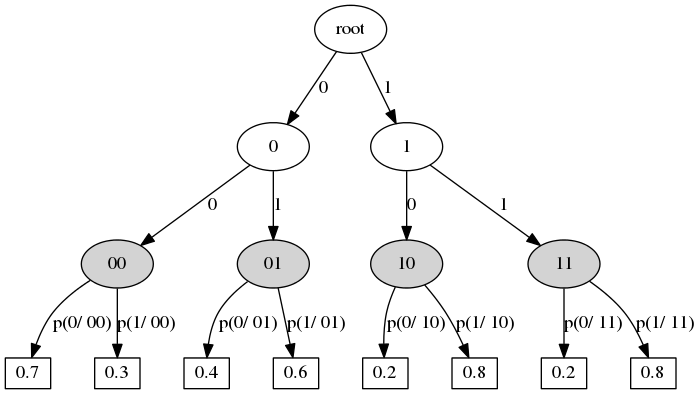
\includegraphics[scale=0.3]{img/Context_trie.png}
	\centering
	\caption{ Контекстное дерево переходов Марковского процесса порядка 2 }
	\label{ris:context_trie}
	
\end{minipage}
\hfil \hfil
\begin{minipage}[b]{0.49 \textwidth}
	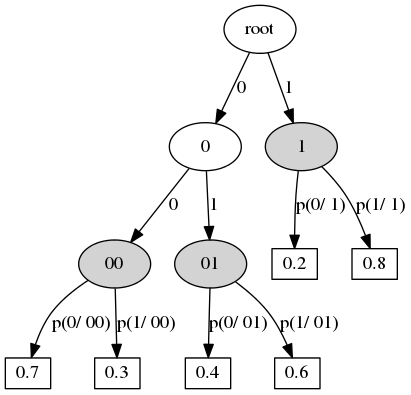
\includegraphics[scale=0.3]{img/Prune_c_trie.png}
	\centering
	\caption{ Подрезанное контекстое дерево }
	\label{ris:prune_c_trie}
\end{minipage}
\end{figure}

Заметим, что в примере \ref{ris:context_trie}, имея для некоторого состояние $x_{t}$, контекст  <<$1$>> , необходимость уточнять его (т.е. спускаться дальше к листу) отсутствует, т.к. распределение на контекстах  <<$10$>>  и  <<$11$>>  одно и тоже. 
Таким образом подстриженное дерево с рисунка \ref{ris:prune_c_trie} задает такие же распределения переходов как и дерево с рисунка \ref{ris:context_trie}. 
Однако второе контекстное дерево имеет разные длины главных контекстов, по этому не один Марковским процесс фиксированного порядка напрямую его использовать не может.
Определим процесс, который может иметь распределение переходов в виде такого дерева.

Будем называть контекстное дерево \textit{правильным}, если все его внутренние узлы имеют ровно по 2 ребенка.

Процесс, переходы которого задаются правильным контекстным деревом, а листья задают распределения на контекстах, и $\pi$ - распределение на листьях,  называется \textit{Марковским процессом переменного порядка} (ММПП).
При этом максимально-возможный порядок ММПП (т.е. максимальная длина контекстов) будем фиксировать (и обозначать тоже за $ m $).

Можно заметить, что ММПП -- это обобщение всех скрытых Марковских процессов порядка меньше либо равного, чем $ m $.

\subsection{Скрытые Марковские модели}
Представим, что каждое состояние Марковского процесса тоже имеет некоторое вероятностное распределение (например, еще одну монетку, или подкошенный \infty-гранник, или распределение Пуассона)

Тогда, имея Марковскую цепь $X = \{x_{t}\}_{t \in Z_{+}}$ и покоординатно определяя для каждого состояния $x_{t}$ новую случайную величину $Y_{t}$ согласно распределению $P(.|~x_{t})$, можно задать породить цепь
$Y = \{y_{t}\}_{t \in Z_{+}}$ .

Процесс, порождающий такую цепь по некоторой Марковской цепи порядка $m$, называется \textit{скрытым Марковским процессом порядка $m$}. 
\\
$ X $ --- \textit{скрытые состояния}, $Y$ --- \textit{наблюдения}.

Итого, \textit{скрытая Марковска модель} (СММ) порядка $ m $ имеет следующие параметры: множество переходов $ A = \{a(q, x^{m})\}_{q \in S, x^{m} \in S^{m}}$, начальное распределение $\pi$ и множество распределений испусканий $ B = \{b(y,x)\}_{y \in R^{l}, x \in S}$, где $ b(y; x) = P(y|x)$. 

Аналогично, \textit{скрытая Марковска модель переменного порядка} (СММПП) задается Марковской моделью переменного порядка (конечное множество контекстов $ C=\{c_{i}\}_{i} $, где $ c_{i} $ - листья некоторого правильного контекстного дерева, распределения на листьях $ A = \{a(q; c)\}_{q \in S, c \in C}$, начальное распределение $ \pi $)  и множеством распределений испусканий $ B = \{b(y,x)\}_{y \in R^{l}, x \in S}$, где $ b(y; x) = P(y|x)$. 

Заметим, что все определяется аналогично, будь у нас множество состояний $ S $ не из двух элементов, а из $n$.
\subsection{Обучение модели СММПП}
{\large Задача:} 
\\
По цепи наблюдений $ Y = (y_{1}, ... y_{T}) $ найти параметры $\Lambda = (A,B,C,\pi)$ модели СММПП, которые бы максимизировали правдоподобие модели, минимизируя при этом длины контекстов. 
\footnote{Параметр алгоритма $ \epsilon $ определяет допустимое отклонение распределений}
\\
Другими словами, найти
\\
$$\Lambda = \arg\!\min_{\Lambda}{\{|\Lambda(C)|\;|\Lambda \in \arg\!\max_{\Lambda}{\{P(Y|\Lambda)\}}\}}$$
\\\\
{\large Алгоритм:}
\\
Параметры алгоритма: 
$ m $ - максимальная длина контекста, 
$ \epsilon_{EM} $ - барьер для остановки EM,
$ \epsilon_{prune} $ - барьер для обрезания дерева
\\
\begin{enumerate}
\item Инициализация контекстов.
$$ C = \{c| c\in S^{m}\}$$
множество из всех строк длины $m$.
\\
Начальные распределения переходов произвольные.
\footnote{В определенных случаях (Gauss, Poisson) частотное распределение, полученное из цепи алгоритмом k-means (k=m), ускоряет работу}
\\
\item EM (Expectation–Maximization algorithm).
\\
Пересчет производится подобно алгоритму Баума-Велша для СММ \cite{Rabiner1989}.
\\
\begin{enumerate}
\item E-шаг (Expectation)
Вводятся дополнительные параметры:
$$ \alpha_{t}(c) = P(y_{0}^{t}, c(x_{t})=c| \Lambda)$$
вероятность породить первые $t+1$ наблюдений равными $y_{0}^{t}$, имея главным контекстом  скрытого состояния $x_{t}$ контекст $ c $, из модели СММПП с параметрами $\Lambda$
\\
$$ \beta_{t}(c) = P(y_{t+1}^{T}| c(x_{t})=c, \Lambda))$$
вероятность того, что последние $T-t$ наблюдений цепи длины $T$, порожденной из модели СММПП с параметрами $\Lambda$, в которой главный контекст скрытого состояния $x_{t}$ является $ c $, совпадают с $y_{t+1}^{T}$
\\
$$ \gamma_{t}(c) = P(x_{t}=c|Y,\Lambda) $$ 
вероятность того, что породив цепь $Y$ моделью СММПП c параметрами $\Lambda$,
главный контекст скрытого состояния $ x_{t} $ является $c$. 

Зная параметры модели, нововведенные параметры считаются следующим образом:
\begin{center}
$$ \alpha_{0}(c) = \pi(c)b(y_{0},c)$$ 
$$ \alpha_{t+1}(c) = \sum_{q \in S, c'=C(cq)}{\alpha_{t}(c')a(c[0];c')b(y_{t+1},c[0])}$$
\\
$$ \beta_{T}(c) = 1$$ 
$$ \beta_{t}(c) = \sum_{q \in S, c'=C(qc)}{a(q;c)b(y_{t+1}, c'[0])\beta_{t+1}(c')}$$
$$p = P(Y|\Lambda) = \sum_{c \in C}\alpha_{T}(c)$$
правдоподобие модели
\\ 
$$ \gamma_{t}(c) = \frac{\alpha_{t}(c)\beta_{t}(c)}{p}$$
\end{center}
\item M-шаг (Maximization)
На этом шаге, алгоритм обновляет параметры модели максимизируя правдоподобие, при условии посчитанных $\alpha, \beta, \gamma$;

Для пересчета множества распределений переходов вводится еще один дополнительный параметр $\xi$\\
$ \xi_{t}(q;c) = P(c(x_{t})=c, x_{t+1} = q| Y, \Lambda)$ ---
вероятность того, что породив цепь $Y$ моделью СММПП c параметрами $\Lambda$, 
главный контекст скрытого состояния $ x_{t} $ является $c$ и состояние $ x_{t+1} $ совпадает с $q$
$$ \xi_{t}(q;c) = \frac{\alpha_{t}(c)a(q;c)b(y_{t+1},q)\beta_{t+1}(qc)}{p} $$
\\
Обновление $ A $ по $ \xi $\\
$$ a(q; c) = \frac{\sum_{t}\xi_{t}(q,c)}{p(c)}$$
Обновление $\pi$
$$\pi(c) = \sum_{t}\gamma_{t}(c)$$

Пересчет $ B $ зависит от принятого семейства моделей испусканий и производится с помощью $ \gamma $ в точности также как и в алгоритме Баума-Велша.
В случае распределения Пуассона
$b(.~|~c) \~ Poisson(\lambda_{c})$ 
пересчет параметров происходит следующим образом
$$ \lambda_{c} = \frac{\sum_{t}{\gamma_{t}(c)y_{t}}}{\sum_{t}{\gamma_{t}(c)}}$$
\end{enumerate}
EM-алгоритм запускает поочередно E-шаг и M-шаг, пока правдоподобие с предыдущей итерации отстает от правдоподобия с текущей итерации более, чем на $ \epsilon_{EM}$
(т.е. пока итерация дает значимый прирост правдоподобия)
\item Обрезание дерева.
Если существует внутренний лист контекстного дерева $ s $ такой, что 
$$ \forall q \in S \; P(sq)kl(sq, s) < \epsilon_{prune} $$
(дети не уточняют родителя), то $ s $ становится листом, а все его потомки обрезаются.
$$kl(u, w) = \sum_{q' \in S} P(q'|u) log\frac{P(q'|u)}{P(q'|w)}$$
расстояния Кульбака-Лейблера для апостериорных распределений.
\item Если на третьем шаге ничего не произошло, то алгоритм заканчивает работу, 
иначе происходит обновление параметра $ A $ для новых контекстов
$$ a(q; c) = P(q| c) $$
и алгоритм переходит на второй шаг (EM-алгоритм).

\end{enumerate}
Обозначения: 
\\
$ c[0] $ - состояние, являющееся началом контекста $ c $
\footnote{Контекст $ c $ представляем как последовательность состояний 
$c[0]c[1]\ldots c[l-1]$, где $ l $ - длина контекста.}
\\
$ c(x_{t}) $ - контекст состояния $ x_{t} $ 
\\
$ C(s) $ - листья, являющиеся потомками $ s $, если $ s $ принадлежит дереву 
\\
$ C(s) $ - контекст максимальной длины, являющийся префиксом $ s $, если $ s $ не принадлежит дереву 
\\\\
\textbf{Замечание.}  Вероятностные переходы на главных контекстах задают вероятностные переходы на всем дереве
$$ p(q|s) = \frac{\sum_{c \in C(s)} {p(q|c)p(c)}}{\sum_{q'}\sum_{c \in C(s)} {p(q'|c)p(c)}} $$ 
\\\\\
\textbf{Замечание.} При пересчете вероятности могут очень близко подходить к нулю, что негативно влияет на точность расчета. Для избежания этой проблемы все расчеты следует проводить не с вероятностями, а с логарифмами от них.
\\\\\
\textbf{Замечание.} EM следует запускать несколько раз, т.к. он может застревать в локальных максимумах функции правдоподобия.

\subsection{Обучение на нескольких выборках}
В случае пропусков или разрывов в наблюдениях, обучение модели может проходить на множестве из нескольких цельных кусков.
\\
Более формально задачу можно описать так: 
\\
пусть дано $ N $ выборок $ \{Y^{1} \ldots Y^{N}\}$ подчиненных единому скрытому Марковском процессу переменного порядка, требуется найти параметры модели $\Lambda$ максимизирующие общее правдоподобие 
$$P(Y^{1} ... Y^{N}| \Lambda) = \prod_{i}{P(Y^{I}|\Lambda)}$$
в классе рассматриваемой модели.
\\
Приведем небольшие корректировки алгоритма выше для решения этой задачи
\\
EM-алгоритм
\begin{enumerate}
\item Expectation
Считаем для каждой выборки  $\alpha^{d}, \beta^{d}, \gamma^{d}, \xi^{d}$
\\
Общая $\gamma$ - конкатенация гамм на выборках
$$ \gamma = [\gamma^{1}, \ldots ,\gamma^{N}] $$
\\
$ p = \prod_{d}{p^{d}}$
\item Maximization
$$ a(q;c) = \frac{\sum_{d}{\sum_{t}{\xi^{d}_{t}(q;c)}}}{\sum_{t}{\gamma_{t}(c)}} $$
нормировка
$ a(q;c) = \frac{a(q;c)}{\sum_{q}{a(q;c)}} $
\end{enumerate}

\subsection{Сравнение}
Чем больше параметров у модели, тем лучше она подстраивается под данные, и тем проще переобучается. 
По этому, при сравнении моделей обученных на одних и тех же данных со схожим правдоподобием, предпочтительней будет та, которая имеет меньшее число степеней свобод или параметров. 
Конкретную величину, которую следует сравнивать для моделей обученных на одинаковых данных, предлагает критерий Акаике (AIC).
$$ AIC = 2k-2log(L) $$ 
где $ k $ - число параметров модели, $ L $ - максимальное правдоподобие модели на заданной выборке. Чем $AIC$ меньше, тем модель лучше. 

Количество степеней свободы для СММ $ m $-го порядка c $ n $ скрытыми состояниями и Пуассоновскими испусканиями можно посчитать как
\\
$k$ = [количество степеней свободы $ A$ ]
$+$ [количество степеней свободы $ B $] $+$ [количество степеней свободы $ \pi $] =
\\= $n^m(n-1)\;+\;n\;+\;(n^m-1)$ = 
\\= $n^{m+1} + n - 1$
\\
При $n=2$, $k=2^{m+1} + 1$ 

Количество степеней свободы для СММПП с $n$ скрытыми состояниями, $l$ контекстами, максимально-возможным порядком $m$ и Пуассоновскими испусканиями =
\\= $l(n-1)\;+\;n\;+\;(l-1) + 1$ = 
\\= $n(l+1)$
\\
При $n=2$, $k=2(l+1)$ 
\\
Последняя единичка -- это параметр задающий вид дерева.

Видно, что если сравнивать СММ порядка $m$ и эквивалентную ей СММПП (т.е. $l = n^{m}$), то количество параметров у второй окажется на один больше, в остальных же случаях СММПП имеет меньшее количество параметров, и, при схожем правдоподобии выигрывает по критерию Акаике.


\section{Реализация}
Алгоритм обучения скрытой Марковской модели переменного порядка был реализован на языке программирования Python. 
\\
Критическим по производительности является E-шаг, он был перенесен на Cython.
\\
Основные использованные библиотеки.
\begin{itemize}
\item
NumPy, SciPy для операций над матрицами.
\item
Joblib для распараллеливания по потокам.
\\
В случае обучения на нескольких выборках, E-шаг для каждой выборки считается независимо, по этому эту часть можно параллелить.
\item
Pygraphviz для отрисовки деревьев. 
\item
Matplotlib для отрисовки графиков.
\end{itemize}

\section{Применение}
\subsection{Проверка на смоделированных данных}
План проверки работы СММПП.
\begin{enumerate}

\item
Генерация параметров $ \Lambda $ начальной модели СММПП.
\item
Порождение выборки $ Y $ из заданной модели.
\item
Обучение новой модели на $ Y $, получение предсказанных параметров $\hat{\Lambda}$.
\item
Сравнение параметров $ \Lambda $ и $ \hat{\Lambda} $.
\end{enumerate}

Ниже приведены три примера теста.
\\Первый проверяет работу модели для смеси (СММ 0-го порядка), второй --- для СММ первого порядка, третий для модели СММПП, не являющейся СММ фиксированного порядка.
\begin{itemize}
\item Смесь.
\begin{enumerate}
\item Параметры начальной модели: $\Lambda = (C, A, B)$ 
\\множество контекстов $C = \{""\}$, множество переходов $A = \{[0.4, 0.6]\}$ (контекстное дерево изображено на рисунке \ref{ris:sample_mixture_real_trie}), множество распределений испусканий $B = \{Poisson(2), Poisson(10)\}$. 
\item Выборка длиной $ T = 5000 $
\item Обучение проходило начиная с полного дерева глубиной $ m  = 4$, и распределением переходов инициализированным алгоритмом k-means. 
\\Остальные параметры алгоритма: барьер для обрезания $ \epsilon_{prune} = 0.007$, барьер для остановки EM $ \epsilon_{EM} =  0.01 $      
\item  На рисунке \ref{ris:sample_mixture_predicted_trie} изображено предсказанное контекстное дерево. 
\\
\\Параметры предсказанной модели $\hat{\Lambda} = (\hat{C}, \hat{A}, \hat{B})$  
\\$\hat{C} = \{""\}, \hat{A} = \{[0.41, .59]\}, \hat{B} = \{Poisson(2), Poisson(10.1)\}$.
\\Параметры исходной и предсказанной модели идентичны.
\begin{figure}[h!]\centering
\begin{minipage}[b]{0.49 \textwidth}
	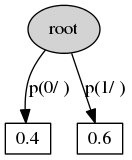
\includegraphics[scale=0.57]{img/sample_mixture/real_trie_.png}
	\centering
	\caption{ Реальное дерево }
	\label{ris:sample_mixture_real_trie}
\end{minipage}
\hfil \hfil%раздвигаем боксы по горизонтали
\begin{minipage}[b]{0.49 \textwidth}
	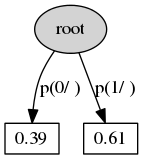
\includegraphics[scale=0.57]{img/sample_mixture/predicted_trie.png}
	\centering
	\caption{ Предсказанное дерево }
	\label{ris:sample_mixture_predicted_trie}
\end{minipage}
\end{figure}
\end{enumerate}
\item СММ порядка 1.
\begin{enumerate}
\item Параметры начальной модели: контекстное дерево -- рисунок \ref{ris:sample_hmm2_real_trie}, 
\\$B = \{Poisson(1), Poisson(8)\}$. 
\item Выборка длиной $ T = 5000 $
\item Параметры обучение те же, что и примером выше.      
\item Предсказанное контекстное дерево -- рисунок \ref{ris:sample_hmm1_predicted_trie}, 
$\hat{B} = \{Poisson(1), Poisson(8)\}$
\\Параметры исходной и предсказанной модели идентичны.
\\Рисунок \ref{ris:sample_hmm1_log_likelihood} -- график логарифма правдоподобия по всем итерациям обучения. Грубо говоря, это карта обучения. На ней видно, как сначала алгоритм 6 итераций EM обучался на 16 контекстах, после чего дерево подстриглось до 2 контекстов. Следующему EM не удалось значимо увеличить прадоподобие модели, поэтому на третей итерации он закончил работу. Далее дерево не удалось еще раз подрезать, поэтому весь алгоритм закончил свою работу (это видно из отсутствия следующего бокса под график ЕM).
\begin{figure}[h!]\centering
\begin{minipage}[b]{0.49 \textwidth}
	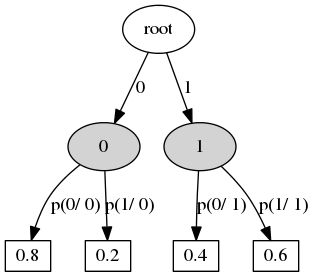
\includegraphics[scale=0.4]{img/sample_hmm1/real_trie_.png}
	\centering
	\caption{ Реальное дерево }
	\label{ris:sample_hmm1_real_trie}
\end{minipage}
\hfil \hfil%раздвигаем боксы по горизонтали
\begin{minipage}[b]{0.49 \textwidth}
	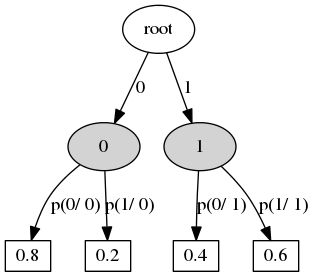
\includegraphics[scale=0.4]{img/sample_hmm1/predicted_trie.png}
	\centering
	\caption{ Предсказанное дерево }
	\label{ris:sample_hmm1_predicted_trie}
\end{minipage}
\begin{minipage}[b]{0.49 \textwidth}
	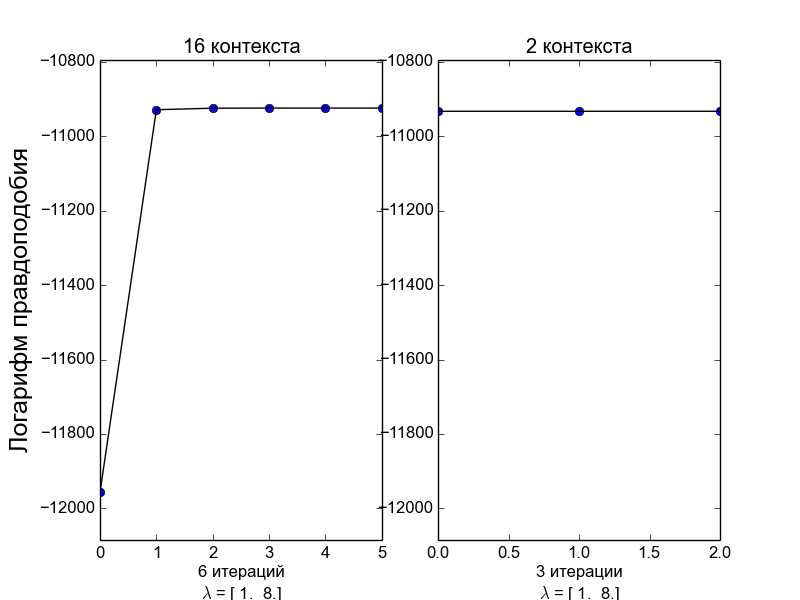
\includegraphics[scale=0.4]{img/sample_hmm1/plot_.png}
	\centering
	\caption{ Карта обучения }
	\label{ris:sample_hmm1_log_likelihood}
\end{minipage}
\end{figure}
\end{enumerate}
\item Более интересны случай, СММПП
\begin{enumerate}
\item Параметры начальной модели: контекстное дерево -- рисунок \ref{ris:sample_real_trie}, \\$B = \{Poisson(3), Poisson(15)\}$. 
\item Выборка длиной $ T = 5000 $
\item Параметры обучение те же, что и примерами выше.      
\item Предсказанное контекстное дерево -- рисунок \ref{ris:sample_predicted_trie}, 
$\hat{B} = \{Poisson(3.1), Poisson(15)\}$
\\Параметры исходной и предсказанной модели идентичны.
\\
Рисунок \ref{ris:sample_log_likelihood} -- карта обучения.
\begin{figure}[h!]\centering
\begin{minipage}[b]{0.49 \textwidth}
	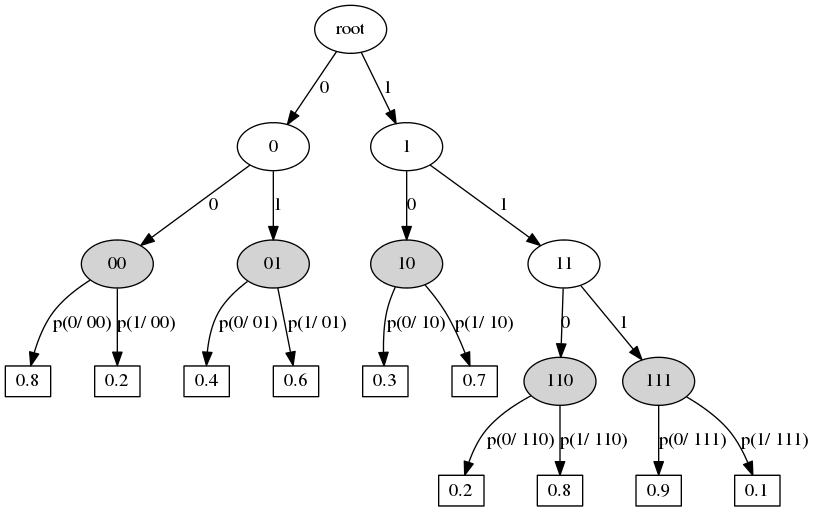
\includegraphics[scale=0.3]{img/sample/real_trie_.png}
	\centering
	\caption{ Реальное дерево }
	\label{ris:sample_real_trie}
	
\end{minipage}
\hfil \hfil%раздвигаем боксы по горизонтали
\begin{minipage}[b]{0.49 \textwidth}
	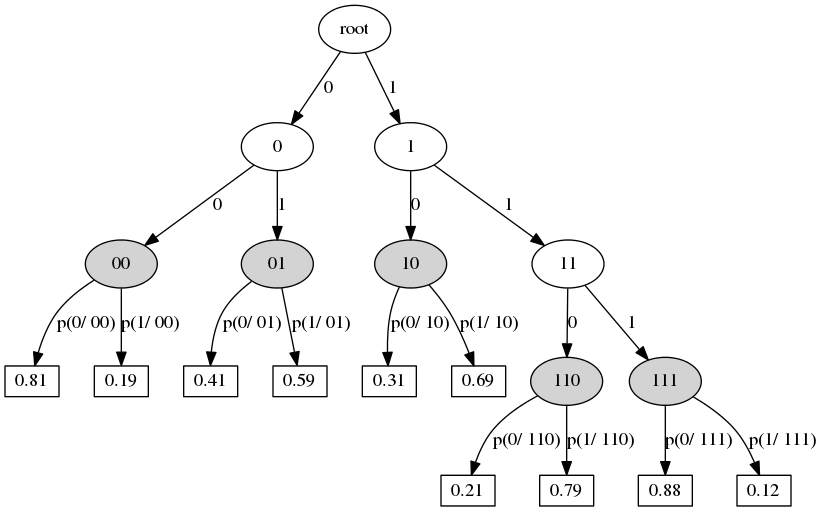
\includegraphics[scale=0.3]{img/sample/predicted_trie.png}
	\centering
	\caption{ Предсказанное дерево }
	\label{ris:sample_predicted_trie}
\end{minipage}
\begin{minipage}[b]{0.8 \textwidth}
	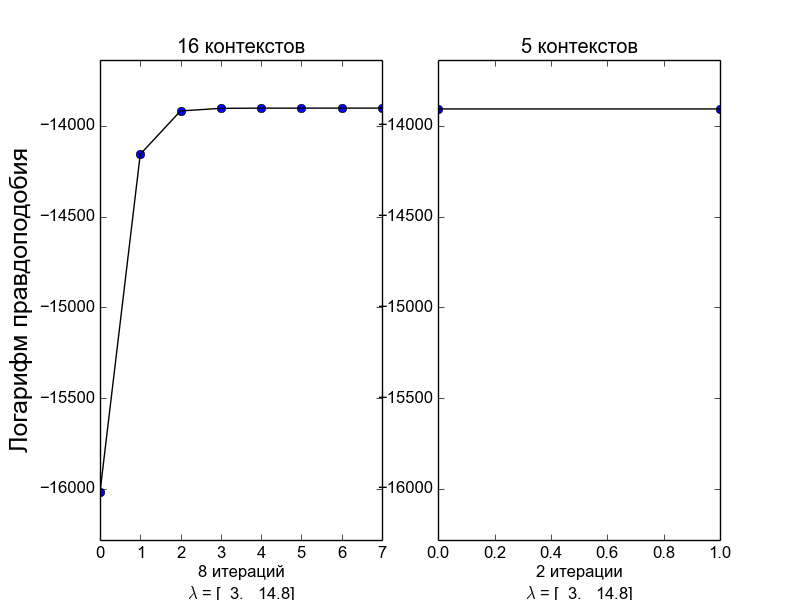
\includegraphics[scale=0.4]{img/sample/plot_.png}
	\centering
	\caption{ Карта обучения }
	\label{ris:sample_log_likelihood}
\end{minipage}
\end{figure}
\end{enumerate}
\end{itemize}


\subsection{ChIP-seq, реальные данные}
Данные были взяты из проекта ENCODE (ENCyclopedia of DNA Elements).
В качестве исследуемого белка был выбран гистон H3 с ацетилированным лизином в 27-й позиции хвоста. Рассматриваемые клетки --- эмбриональные стволовые клетки человека \cite{ENCODE}.
Размер окна был выбран равный 200 п.н.

В качестве выборок были рассмотрены ненулевые участки вектора, полученного после деления результата эксперимента ChIP-seq на окна. 

Параметры обучения:\\
Начальная глубина дерева $= 6 $.
$\epsilon_{prune} = 0.04$,
$\epsilon_{em} = 0.05$
\begin{figure}[h!]\centering
\begin{minipage}[b]{0.49 \textwidth}
	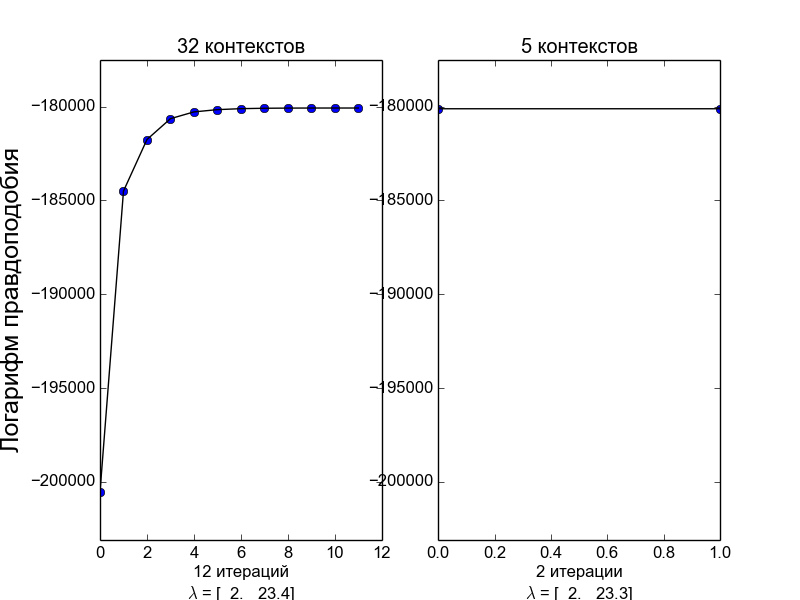
\includegraphics[scale=0.47]{img/real/plot_.png}
	\centering
	\caption{ Карта обучения }
	\label{ris:log_likelihood}
\end{minipage}
\hfill
\begin{minipage}[b]{0.32 \textwidth}
	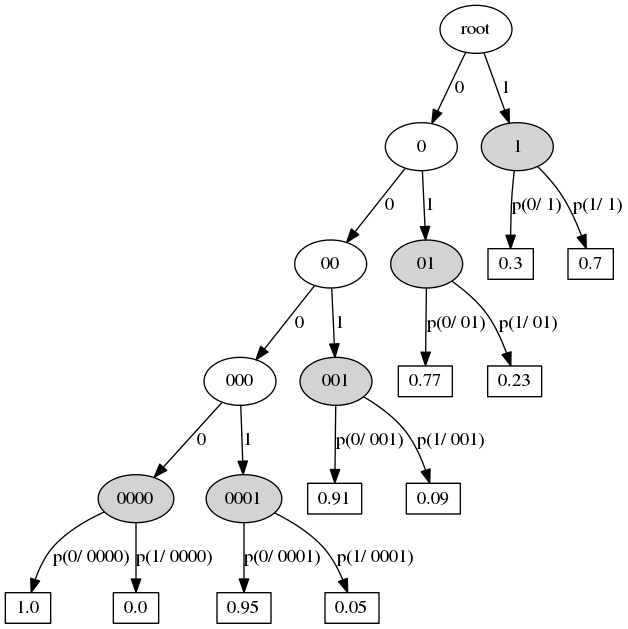
\includegraphics[scale=0.29]{img/real/predicted_trie.png}
	\centering
	\caption{ Контекстноe дерево }
	\label{ris:real_trie}
\end{minipage}
\end{figure}

Рисунок \ref{ris:log_likelihood} показывает, что сначала алгоритм 12 итераций EM обучался на 32 контекстах, потом подрезал дерево до 5 контекстов. После чего ни обучение, ни подрезание не дало результатов, поэтому, алгоритм закончил работу.

Рисунок \ref{ris:context_trie} показывает получившееся контекстное дерево.

Приведем таблицу сравнения для СММПП, СММ5 (СММ 5-го порядка, соответствует дереву, с которого мы начали обучения)и СММ (СММ 1-го порядка, именно его чаще всего используют для анализа данных ChIP-seq)
\begin{figure}[h!]\centering
\begin{minipage}[b]{0.32 \textwidth}
	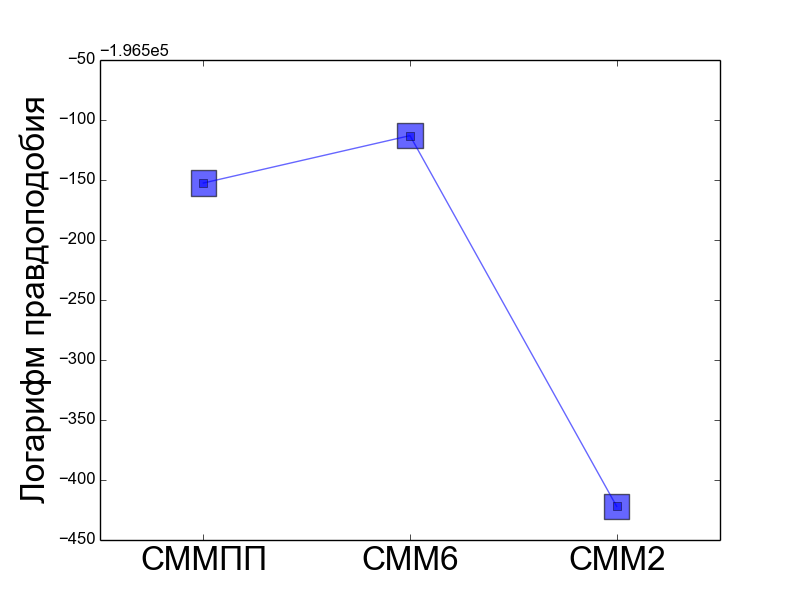
\includegraphics[scale=0.28]{img/real/log_p.png}
	\centering
	\caption{ Сравнение логарифма правдоподобия}
	\label{ris:real_comp_log_p}
\end{minipage}
\hfill
\begin{minipage}[b]{0.32 \textwidth}
	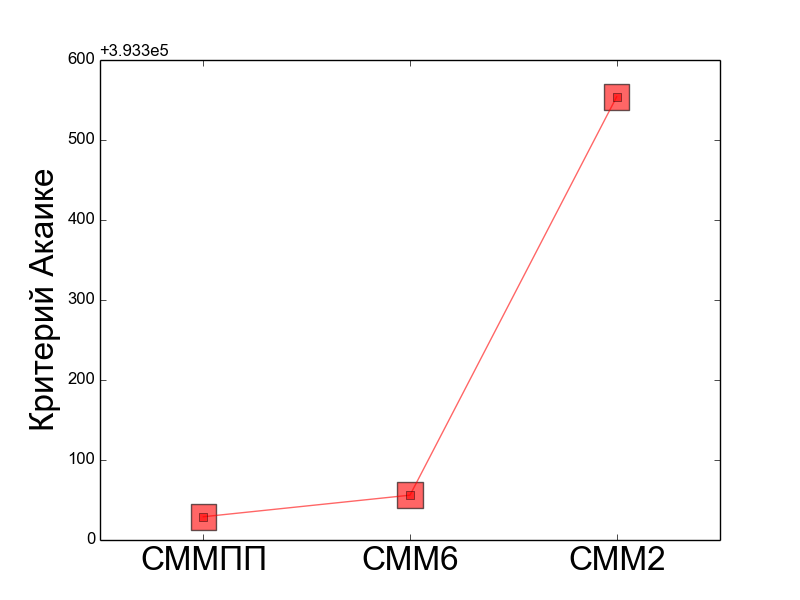
\includegraphics[scale=0.28]{img/real/aic.png}
	\centering
	\caption{ Сравнение критерия Акаике }
	\label{ris:real_comp_aic}
\end{minipage}
\hfill
\begin{minipage}[b]{0.32 \textwidth}
	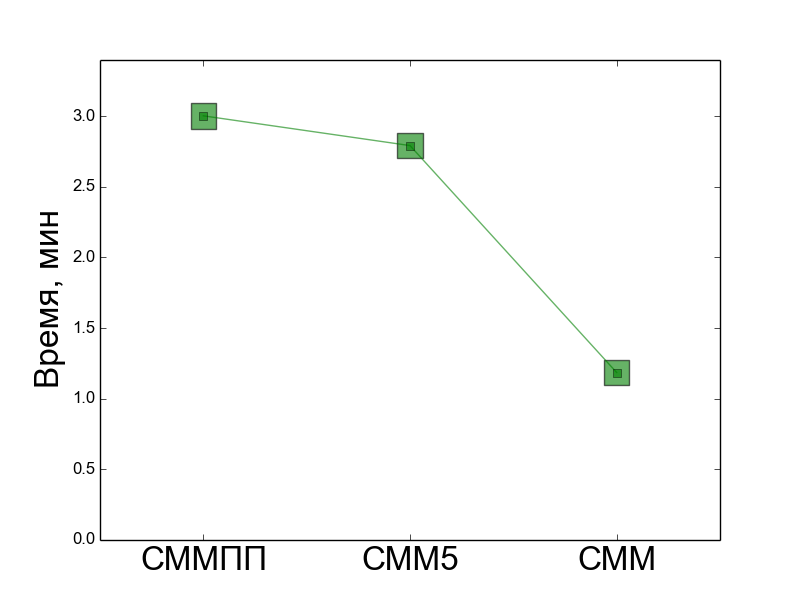
\includegraphics[scale=0.28]{img/real/time.png}
	\centering
	\caption{ Сравнение времени обучения }
	\label{ris:real_comp_time}
\end{minipage}
\end{figure}

На рисунке \ref{ris:real_comp_log_p} приведено сравнение правдоподобия моделей (в логарифмической шкале). Видно, что СММ5 лидирует. Однако СММПП ей не сильно уступает по сравнению с СММ.

Интересный результат показал критерий Акаике. Напомним, что данный критерий, чем меньше тем лучше. Сравнение его изображено на рисунке \ref{ris:real_comp_aic}.
Хотя СММ2 имеет гораздо меньшее количество параметров, чем СММПП, правдоподобие ее невилико, по этому по критерию Акаике она проигрывает. И наоборот, хотя СММ6 имеет лучшее среди этих трех моделей правдоподобие, оно имеет слишком много параметров, поэтому СММПП по критерию Акаике выигрывает и ее.

Рисунок \ref{ris:real_trie} показывает сравнение времени обучения. Тут СММПП дает похожий результат с СММ6, немного ей уступая. СММ, в силу того, что она имеет более простую структуру, обучается быстрее всех.


\section*{Заключение}
В ходе работы были решены поставленные задачи.
\begin{enumerate}
\item
Проанализированы существующие скрытые Марковские
модели переменного порядка, разработана и
реализована подходящая под данные ChIP-seq модель.
\item
Проведен анализ эффективности работы модели на
синтетических данных, сравнение с более простыми
моделями (СММ первого порядка, пятого), осуществлено применение к
данным ChIP-seq
\end{enumerate}


\bibliographystyle{plain}
\bibliography{diploma.bib}
\end{document}
